\documentclass{osu-thesis}

\usepackage{siunitx}
\sisetup{round-mode=places, round-precision=3}

\usepackage{tikz}
\usetikzlibrary{shapes,positioning,matrix}
\usetikzlibrary{automata, positioning, arrows}
\tikzset{->, >=stealth', node distance=3cm, every state/.style={thick, fill=gray!10}, initial text=$ $}

\usepackage{lipsum}

\setfigurepath{Figures}
\setlistingpath{Source}
\addbibresource{References/Example.bib}
% \bibliography{References/Example.bib}



%%%% Packages

\usepackage{graphicx}
\usepackage{algorithm}
% \usepackage{booktabs}
% \usepackage[noend]{algpseudocode}


\usepackage{amsmath}

%%%%


\begin{document}	

\settitle{SELF-TRAINABLE 3D-PRINTED PROSTHETIC HANDS}
\setabstracttitle{SELF-TRAINABLE 3D-PRINTED PROSTHETIC HANDS}
\setauthor{KYUNGHO NAM}
\setdegree{Doctor of Philosophy}
\setmajor{Computer Science}
\setdegreeOne{%
  Bachelor of Science in Electrical Engineering \\
  Oklahoma State University \\
  Stillwater, Oklahoma \\ 2015}
% \setdegreeTwo{%
%   Doctor of Philosophy in Computer Science \\
%   Oklahoma State University \\
%   Stillwater, Oklahoma \\ 2022}
\setgraddate{December, 2022}
\setadvisor{Christopher John Crick}
\setmemberOne{Blayne E. Mayfield}
\setmemberTwo{Nohpill Park}
% \setmemberThree{Member Three}
\setmemberOutside{Guoliang Fan}
\frontmatter
\thetitlepage
\approvalpage
\begin{acknowledgementspage}
I cannot express my gratitude enough to my academic advisor Dr. Christopher John Crick for his continued support and encouragement. I offer my sincere appreciation for the learning opportunities provided by him.
At the end, glory and thanks to the God, the Almighty, for His helps throughout my research life to complete the research successfully.
\end{acknowledgementspage}

\begin{abstractpage}


3D printed prosthetics have narrowed the gap between the tens of
thousands of dollars cost of traditional prosthetic designs and
amputees' needs. However, the World Health Organization estimates that
only 5-15\% of people can receive adequate prosthesis services
~\cite{WHO}. To resolve the lack of prosthesis supply and reduce cost
issues (for both materials and maintenance), this paper provides an
overview of a self-trainable user-customized system architecture for a
3D printed prosthetic hand to minimize the challenge of accessing and
maintaining these supporting devices. In this paper, we develop and
implement a customized behavior system that can generate any gesture
that users desire. The architecture provides upper limb amputees with
self-trainable software and can improve their prosthetic performance
at almost no financial cost.  All kinds of unique gestures that users
want are trainable with the RBF network using 3 channel EMG sensor
signals with a 94\% average success rate.  This result demonstrates
that applying user-customized training to the behavior of a prosthetic
hand can satisfy individual user requirements in real-life activities
with high performance.



\end{abstractpage}

\tableofcontents
\listoftables
\listoffigures
\mainmatter
\pagestyle{osu}
\chapter{Introduction}

Article 25 of the Convention on the Rights of Persons
with Disabilities, adopted by the General Assembly of the United
Nations, establishes the right to receive the highest feasible
standard of health care without discrimination on the basis of
disability from State Parties \cite{UN}. Concerning amputees, the
provision of affordable and high-quality prosthetic aids is a human
rights argument, one that governments must support. Nevertheless,
World Health Organisation figures show that only 5-15\% of the
population in need is able to access prosthetic and orthotic
appliances in today's world \cite{WHO}. The difficulty of accessing
such devices is greater in low- and middle-income countries. In such
areas, charities, often staffed by people who are not trained
professionals, often provide prosthetic and orthotic services, leading
to compromised services and poor quality and fit. In addition, without
adequate provision for maintenance, people are often restricted in
their quality of life, excluded from participating in society, and
locked into poverty and isolation \cite{WHO}. Most amputees who have
any kind of prosthetic hand at all are only able to obtain a cosmetic
hand, which affords a realistic appearance \cite{3D4} but provides
little functionality for grasping objects or anything else.

One of the main issues for useful prostheses is cost. The total mean
life cost for an amputee is reported to be \$509,275
\cite{cost_1}. The weighted average prosthesis price is \$10,232, and
total costs for the prosthesis after the second year are \$181,500
\cite{cost}. The annual maintenance costs for a functional prosthesis
are expected to be 20\% of the initial prosthesis' price, for a total
of \$83,490 after the second year.

Most studies in the field of prosthetics have focused on reducing
acquisition costs and improving performance.  However, maintenance
service for prostheses has not been nearly as heavily studied.
Amputees with prostheses certainly require such ongoing service,
especially as new situations arise.  For instance, child users grow up
and need larger-sized prostheses, and old prosthetics suffer decreased
performance.  To address the necessity of excellent quality
maintenance service and the lack of low-cost, high-performing
prostheses, this paper introduces an architecture that can be
self-trainable and user-customized, based on a very low-cost
3D-printed prosthetic hand. This architecture provides self-trainable
software to the user, which can increase the prosthetic hand's
performance at a very low financial cost. A small amount of time
invested in training the user's prosthesis returns high accuracy in
its performance with repetitive behavior.

\chapter{Literature Review}

\section{3D-printed prostheses}
Currently, only 5-15\% of people who need them have access to
prostheses \cite{WHO}, so much effort and research is going into
expanding the availability of low-cost prosthetics.  Several recent
works \cite{3D4}\cite{3D2} aimed to build a low-cost robotic
prosthetic arm using 3D printing technology with capable and
comfortable design. 3D printing technology suggests a new path to
satisfying amputees' financial needs and various physical conditions,
while also enabling departures from the prosthesis's standard size for
children or veterans with upper limb loss. \cite{3D3} For similar
reasons, in order to minimize the cost of supplying the prosthesis to
more people, a 3D-printed hand was chosen as the basic structure for
this study.

\section{EMG-based human robot interaction}
Electromyography (EMG) \cite{review, EMG} is one of several biological
signals produced by the human body which can be used to predict motor
intentions, in addition to such signals as electrical ultrasound (EOG)
\cite{EOG}, electrical ECG \cite{ECOG}, EEG \cite{EEG_1}, and
brainwaves (MEG) \cite{MEG}. Likewise, many different sensors have
been used to read users' intentions to control their prostheses
\cite{MMG}.  In particular, EMG sensors are available that are both
highly accurate and low cost, and can be used to control diverse
devices. The most attractive aspect of an EMG sensor is that it is a
hands-free sensor that does not require invasive surgery.  EMG
sensors \cite{controlEMG} have been used to control a mouse
\cite{mouse}, a mobile RC car \cite{RCcar}, and even to assemble a
Rubik's cube \cite{rubikcube}.

\section{EEG-based human robot interaction}
Another non-invasive control techniques
that translate imagined hand movements into motor signals use
electroencephalograms (EEGs) \cite{EEG} as Brain-Machine Interfaces.
An EEG-based study work \cite{[???]} developed and validated a neuro-based
method for objectively verifying robot behavior in HRI, and proposed to
detect improper / unexpected / erroneous robot behavior using the
electroencephalogram (EEG) of a human interaction partner.
EEG-based brain-controlled mobile robots can be useful tools for 
severely disabled persons in their daily lives, 
particularly when it comes to assisting them in moving 
voluntarily. \cite{EEG}
This EEG human-robot interaction technique has already been successful
in detecting and classifying simple hand motions. \cite{[???]}



Our research relies on a hand prototype \cite{3D1} which emulates the
structure of a human hand using 5 servo motors and electromyography
(EMG) sensors to detect the electrical potential when muscle
contraction appears.

The novel problem we consider is customizing a cheaply-produced
3D-printed prosthetic device for each diverse user.  A
perfectly fitting prosthesis with high performance for all the
different individuals is impracticable.  Most of the research in the
field of prosthetic hands focused only on reducing cost or improving
performance, while prosthesis maintenance services have not been as
intensely studied.  Adequate after-care maintenance services for
amputees who use the prosthesis are extremely important.  We have
developed an architecture that allows users to train their devices to
have high-performance and creative idiosyncratic behaviors tailored
exactly to their individual use cases.
\chapter{Control system architecture components}
In this section, we provide a detailed description of the individual
control system components of this architecture.

\section{3D-printed prosthetic hand}
Many open-source 3D-printable prosthetic hands are available. All of
our prosthesis parts are defined in stereolithography (STL) files
\cite{STL} with different designs that can be modified for the
best-fitting model for each different user.  Armed with those STL
files, the 3D printer can generate a prosthetic hand with diverse
sizes for different people who need it. For the experiments, an
open-source design was adopted and printed with a 3D printer, which is
easily modified in the future for each user's needs.

In our prosthesis prototype, five MG996R servo motors with a maximum
stall torque of 11 kgf·cm powered by 6V are used as actuators, one for
each finger \cite{3D1}. The motors are controlled by an Arduino Mega
Atmel 8-bit AVR microcontroller. When the EMG sensors detect a muscle
contraction, the microcontroller controls individual servo motors to
control individual fingers in real-time through the decision-making
process. The printed 3D prosthetic hand is shown in Fig. \ref{hand}.

% \begin{figure}[h]
%   \centering
% %   \includegraphics[width=3.0in]{Figures/3dhand3.jpg}
%   \includegraphics[.9\textwidth]{Figures/3dhand3.jpg}
%   \caption{3D-printed prosthetic hand}
%   \label{hand}
% \end{figure}

\singlefigure[.9\textwidth]{hand}{3dhand3.jpg}{3D-printed prosthetic hand}{3D-printed prosthetic hand}


%% Electromyography Signal

\section{Electrical biosignal sensors}

\subsection{Electromyography sensors}

To detect and measure the electrical activity produced by muscle
contraction, the electrodiagnostic technique is considered as an input
for the decision-making process. The MyoWare Muscle Sensor is used,
which is designed for microcontroller applications \cite{myo} with the
dimension of 52.3x20.7mm.  It needs a voltage power between 2.9-5.7 V
with a maximum current of 14mA. As shown in Fig. \ref{myo}, the sensor
can measure the muscle's electrical potential with three electrodes
when the sensor board is placed at the skin above the targeted muscle.

% \begin{figure}[h]
%   \centering
%   \includegraphics[width=3.4in]{Figures/myosensor.png}
%   \caption{The layout of the MyoWare Muscle Sensor (AT-04-001)}
%   \label{myo}
% \end{figure}

\singlefigure[.9\textwidth]{myo}{myosensor.png}{The layout of the MyoWare Muscle Sensor (AT-04-001)}{The layout of the MyoWare Muscle Sensor (AT-04-001)}

\subsection{EMG signal processing}

The MyoWare Sensor can detect envelope EMG and raw EMG with the
voltage signal difference between the central muscle electrode and the
reference electrode. The sensor generates the envelope signal, which
is amplified, rectified, and integrated within the sensor transducer,
as shown in Fig. \ref{signal}. The signal amplitudes are translated
through the microcontroller's analog-to-digital converter (ADC), and
are then utilized as features to select human behaviors at the
decision-making process.

% \begin{figure}[h]
%   \centering
%   \includegraphics[width=3.2in]{Figures/signals.png}
%   \caption{An example of EMG signals processing}
%   \label{signal}
% \end{figure}

\singlefigure[.9\textwidth]{signal}{signals.png}{An example of EMG signals processing}{An example of EMG signals processing}




\subsection{Electroencephalogram sensors}
Electrodes placed on your scalp detect tiny electrical charges that
result from the activity of your brain cells to identify and measure
the electrical activity produced by irregularities in your brain
signals or electrical activity of your brain.
The electrodiagnostic approach is used as a source of information
for decision-making.
The Muse S brain sensing headband is used, which is designed for
a multi-sensor brain-computer interface headband that can give you
real-time feedback on your brain waves.

\subsection{EEG signal processing}
The Muse S can detect signals from TP9, AF7, AF8, TP10 in the
international standard EEG placement system. According to the technical manual \cite{[???}, Muse S receives a raw signal ranging from 0 to 1682 microvolts (V), which can represent the raw data of each sensor. Fast Fourier Transform (FFT) of raw data is used to generate discrete frequency values on the log scale. The frequency bands of the brain waves can be determined using a spectrum of discrete frequency data: Gamma (30-44 Hz), Beta (13-30 Hz), Alpha (7.5-13 Hz), Theta (4-8 Hz), and Delta (1-4 Hz). Based on the Power Spectrum Density (PSD) log of EEG data for each channel, this absolute band power is utilized as a function of selecting human behavior in the decision-making process.
% PICTURE
% PICTURE
% PICTURE
\section{Self-training user-customized control software}

In our software designed to train the user's prosthetic hand, all the
magnitude of the envelope signals, generated by 3 channel EMG sensor
signals, were transferred to the Arduino platform. The microcontroller
can read and record all the sensor data as a user history to train
each behavior into the machine. In the trained device, these three
matrix values contain sensor values (0-1000) as inputs, which are used
to produce prosthetic hand behavior decision-making in real-time.  The
training function procedure and the actual operation function
procedure are presented in Algorithm \ref{alg:sysArch}.

% Algorithm
\begin{algorithm}
\caption{System architecture}
\label{alg:sysArch}
\begin{algorithmic}[1]
\Procedure{Training}{}

\State \textit{y.append(CustomGesture)}
\Comment{custom new gesture}
\For {$i=y_{0}$ to $y_{max}$}
    \For {$j=0$:$T$}
        \State $ \textit{$X_{j}^i$} \gets \textit{readSensors()}$
        \EndFor
    \EndFor
\State \textit{clf.fit(X, y)}
\EndProcedure

\Procedure{Movements}{}
\While{$r\not=0$}
\State \textit{ $Gesture = predict(readSensors()) $}
\State \textit{ $MotorController(Gesture, servoMotors())$ }
\EndWhile\label{endwhile}
\EndProcedure
\end{algorithmic}
\end{algorithm}

To train the model, a user's custom gesture is appended (as many as
desired). Each $y$ contains each custom gesture per $T$ iterations,
and each sensor's value is recorded in $X$ for the classification.
The motor outputs provided to move each finger by motor controller
depend on the prediction for the user's specific gesture.

A support vector machine (SVM) \cite{ML1}\cite{ML2} supervised
learning methods, is applied to the prosthetic hand's behavior
classification, with a radial basis function (RBF) kernel. The radial
basic function network has the advantage of solid tolerance to input
noise and is well suited for designing flexible control systems
\cite{RBFAdv}. This gesture classification uses multiple EMG sensors
as input matrix $X$, and the output matrix $y$ consists of each
different individual intended gesture.

The equation \eqref{kernel} defines the radial basis function kernel
for two different inputs $X$ and $X'$, designated as feature vectors,
which is the factor to predict purposing action with trainable
high-performance accuracy.
\begin{equation}
K(X,X') = \exp(-\frac{\lVert X - X' \rVert^2}{2\sigma^2})
\label{kernel}
\end{equation}

The squared Euclidean distance between the two feature vectors is
shown in $\lVert X - X' \rVert^2$.  The $\sigma$ worked as a parameter
condition.


%%% NO NEED TO EXPLAIN
The artificial neural network interpretation of SVMs using radial basis function kernel to train the prosthesis is demonstrated in Fig. \ref{RBF}.

%% RBF figure
\begin{figure}[htp]
% \begin{figure}[t]
\centering
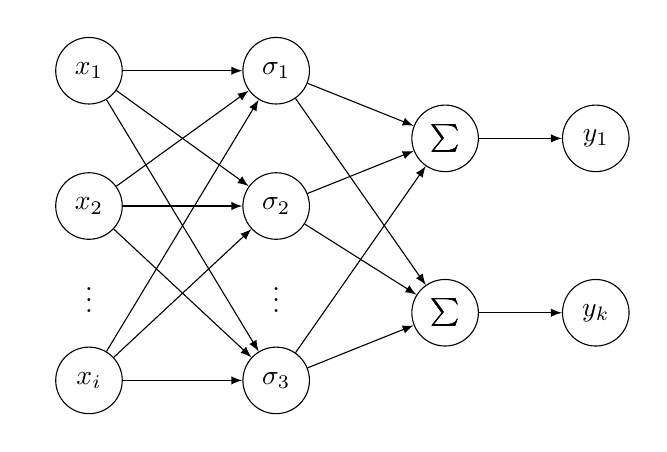
\begin{tikzpicture}[
plain/.style={
  draw=none,
  fill=none,
  },
net/.style={
  matrix of nodes,
  nodes={
    draw,
    circle,
    inner sep=8.5pt
    },
  nodes in empty cells,
  column sep=0.6cm,
  row sep=-11pt
  },
>=latex
]
\matrix[net,row sep=0em, column sep=3em] (mat)
{
             &           \\
  |[plain]|  & |[plain]| &  &         \\
             &           \\
  |[plain]|$\vdots$ & |[plain]|$\vdots$ &  &       \\
             &           \\
};
\foreach \ai in {1,3,5}
  {\foreach \aii in {1,3,5}
    \draw[->] (mat-\ai-1) -- (mat-\aii-2);
}
\foreach \ai in {1,3,5}
  {\foreach \aii in {2,4}
    \draw[->] (mat-\ai-2) -- (mat-\aii-3)node(){$\sum$};
}
\draw[->] (mat-2-3) -- (mat-2-4)node(){$y_1$};
%\draw[->] (mat-2-5)node(){$t_i$} -- (mat-2-4);
 
\draw[->] (mat-4-3) -- (mat-4-4)node(){$y_k$};
% \draw[->] (mat-4-5)node(){$t_k$} -- (mat-4-4);

\node(x1) at (mat-1-1){$x_1$}; \node(s1) at (mat-1-2){$\sigma_1$};
\node(x1) at (mat-3-1){$x_2$}; \node(s2) at (mat-3-2){$\sigma_2$};
\node(x1) at (mat-5-1){$x_i$}; \node(s3) at (mat-5-2){$\sigma_3$};
\end{tikzpicture}
\caption{Radial basis function model}
\label{RBF}

\end{figure}

The support vector classification implementation is tuned with
regularization parameter $C = 2.5$, and the kernel coefficient for RBF
$\gamma = 0.01$ as the best fit.
\chapter{Preliminary Experimentation and results}

In order to evaluate the performance of the architecture, this system
is designed in two different modes, which is depicted in Fig
\ref{layout}.

% \begin{figure}[h]
%   \centering
%   \includegraphics[width=3.5in]{Figures/layout_times.PNG}
%   \caption{Procedures of the system architecture.}
%   \label{layout}
% \end{figure}

\singlefigure[\textwidth]{layout}{layout_times.PNG}{Procedures of the system architecture}{Procedures of the system architecture}

In training mode, when the test subject group performs each different
action, 3 different EMG sensors read the subjects' muscle
contraction. The raw EMG sensor signals are rectified in real-time as
feature values for classification.  In real-life mode, the test
subjects perform the same actions to practically actuate the 3D
printed prosthetic hand. In this mode, sensing, preprocessing, and
feature extraction are processed, the same as in training
mode. However, this real-life mode predicts the subjects' actions
using a trained classification model to generate classification
results. This classification result is transferred to the motor
controller to control each motor assigned with each finger.

The experiments were conducted with $n=7$ test subjects containing 5
males and 2 females in their 20s and 30s. Each subject in the
experiment was instructed to attach three EMG muscle sensors to their
muscles, shown in Fig \ref{pic}.  The group was not composed of
amputees, though such individuals will be recruited for subsequent
experiments.  The placement of the three EMG sensor devices on the
forearm was chosen to accommodate amputees.

% \begin{figure}[h]
%   \centering
%   \includegraphics[width=2.5in]{Figures/am.jpg}
%   \caption{User's unique gesture (Pinky Swear) training with 3 EMG sensors}
%   \label{pic}
% \end{figure}

\singlefigure[.8\textwidth]{pic}{am.jpg}{User's unique gesture (Pinky Swear) training with 3 EMG sensors}{User's unique gesture (Pinky Swear) training with 3 EMG sensors}

The EMG muscle sensors are attached to the area of the flexor
digitorum superficialis, which is an extrinsic flexor muscle that
actuates four fingers with the interphalangeal joints, the flexor
digitorum profundus, which is the muscle that can bend the fingers to
grip, and the flexor pollicis longus, which actuates thumbs,
particularly for writing and painting.

To train various gestures into the prosthetic hand, a trial of using
the prosthetic hand with 3 EMG MyoWare Muscle Sensors was
performed. The subject tried to contract his muscles to perform his
intended hand behavior.  200 samples of EMG sensor data were recorded
during each action.

To testify to the decision-making algorithm's practicality, the
experiment routine is conducted for numerous behaviors, with the EMG
signals used to classify each different hand movement.

Each gesture is repeated, and simultaneously the 200 EMG muscle sensor
values are recorded when the user performs the motion as shown in
Table 1.

\begin{table}[ht]
\caption{Experiments with different actions} % title of Table
\centering % used for centering table
\begin{tabular}{c c} % centered columns (3 columns)
\hline\hline %inserts double horizontal lines
User behavior & Each iteration \\ [0.5ex] % inserts table
%heading
\hline % inserts single horizontal line
Hand Relax & 200 \\ % inserting body of the table
Clenching fist & 200 \\
Open hand & 200 \\
Thumbs up & 200 \\
Pointing somewhere & 200 \\
OK sign & 200 \\
Ball grip & 200 \\
Pencil grip & 200 \\
Smartphone grip & 200 \\
User's unique gesture (whatever the subject wants) & 200 \\ [1ex] % [1ex] adds vertical space
\hline %inserts single line
\end{tabular}
\label{table:nonlin} % is used to refer this table in the text
\end{table}


% \begin{singletable}{table:nonlin}{Experiments with different actions}{Experiments with different actions}

% \begin{tabular}{c c} % centered columns (3 columns)
% \hline\hline %inserts double horizontal lines
% User behavior & Each iteration \\ [0.5ex] % inserts table
% %heading
% \hline % inserts single horizontal line
% Hand Relax & 200 \\ % inserting body of the table
% Clenching fist & 200 \\
% Open hand & 200 \\
% Thumbs up & 200 \\
% Pointing somewhere & 200 \\
% OK sign & 200 \\
% Ball grip & 200 \\
% Pencil grip & 200 \\
% Smartphone grip & 200 \\
% User's unique gesture (whatever the subject wants) & 200 \\ [1ex] % [1ex] adds vertical space
% \hline %inserts single line
% \end{tabular}

% \end{singletable}



Any user's customized unique gestures are recorded in the 'User's
unique gesture (whatever the subject wants),' which can potentially
offer customization for each different user.

Fig. \ref{3dplot} illustrates two representative histories of each EMG
sensor variables' clusters. Each scatter plot color represents a
different labeled gesture. Each axis of the graph shows the actual
sensor variable boundary between 0 to 1000 amplitude, measured by 3
different MyoWare Muscle Sensors.


% \begin{figure*}[h]
%   \centering
%   \includegraphics[width=6.8in]{Figures/pretty_f.png}
%   \caption{Collected 3-channel EMG sensor values for each different action}
%   \label{3dplot}
% \end{figure*}

\singlefigure[.9\textwidth]{3dplot}{pretty_f.png}{Collected 3-channel EMG sensor values for each different action}{Collected 3-channel EMG sensor values for each different action}

The evaluation results of the model are illustrated with a confusion
matrix as shown in Fig. \ref{cm}, which shows the accuracy per user
action label. Each column corresponds to the true label, which is the
user's intended hand gesture, and each row corresponds to the predicted
label, which is the gesture actuated by the prosthetic hand.

% \begin{figure}[h]
%   \centering
%   \includegraphics[width=3.1in]{Figures/confusionmatrix3.PNG}
%   \caption{Confusion matrix represents the accuracy per user action label}
%   \label{cm}
% \end{figure}

\singlefigure[.8\textwidth]{cm}{confusionmatrix3.PNG}{Confusion matrix represents the accuracy per user action label}{Confusion matrix represents the accuracy per user action label}

This equation \eqref{eq} is merely equivalent to the relationship of
predictions that the model classified precisely.

\begin{eqnarray}
  Accuracy & = & \frac{\textit{The number of correct predictions}}{\textit{Total number of predictions}} \\[1ex]
   & = & \frac{\textit{TP + TN}}{\textit{TP + TN + FP + FN}}
    \label{eq}
\end{eqnarray}


The average success rate for all subjects without noise was 94.96\% on
the training set and 91.58\% on the test-set. The best-case subject's
training set estimated accuracy was 95.69\% and the test set
estimated accuracy was 95.50\% as shown in Table 2. The impressive
point of this experiment was the unique gesture at the last part of
the experiment cycle.  As the last step of the experiment, users were
allowed to demonstrate any kind of creative unique gesture such as
crossed fingers, a V-for-victory sign, a finger gun, or the sign of
the horns.  The prosthetic hand successfully captured these gestures
with a high percentage (94\%).



\newcommand{\ra}[1]{\renewcommand{\arraystretch}{#1}}
% \begin{table}[h]
\tabcolsep=0.11cm
\begin{table*}
\footnotesize

\caption{Average recognition success rates of the trained RBF network, linear SVM network, and MLP network}
\centering
\ra{1.3}
\begin{tabular}{@{}rrrcrrcrr@{}}\toprule
\hline\hline %inserts double horizontal lines
& \multicolumn{2}{c}{$RBF$} & \phantom{abc}& \multicolumn{2}{c}{$Linear SVM$} &
\phantom{abc} & \multicolumn{2}{c}{$MLP$}\\
% \cmidrule{2-4} \cmidrule{6-8} \cmidrule{10-12}
$Subject$ & $Training$ $set$ & $Test$ $set$ && $Training$ $set$ & $Test$ $set$ && $Training$ $set$ & $Test$ $set$\\ \midrule
\hline
$without$ $noise$ $=$ $1$ & 95.69\% & 95.50\% && 88.25\% & 89.25\% && 90.50\% & 89.50\%\\
$2$ & 92.00\% & 90.00\% && 90.44\% & 89.50\% && 84.50\% & 84.50\%\\
$3$ & 97.19\% & 89.25\% && 89.19\% & 86.50\% && 87.44\% & 83.00\%\\
\hline
$with$ $noise$ $=$ $4$ & 92.06\% & 80.75\% && 79.25\% & 77.00\% && 68.38\% & 67.25\%\\
$5$ & 82.25\% & 80.50\% && 77.00\% & 73.50\% && 70.25\% & 68.50\%\\
$6$ & 88.44\% & 75.75\% && 68.94\% & 71.25\% && 65.06\% & 69.75\%\\
$7$ & 88.56\% & 83.25\% && 67.69\% & 67.50\% && 64.75\% & 62.25\%\\



\bottomrule
\hline
\end{tabular}

\end{table*}
% \end{table}

When measuring EMG sensors, sometimes sensor values bounce with
subjects' extreme actions.  This noise makes it difficult to obtain
sustainable high-quality electromyography signals for the long term
without tightening the sensor on the arm.  To record an undisturbed
sensor signal, a more elaborate connection apparatus is needed than
the prototype model possessed.  This would further improve the
system's accuracy.

As shown in Fig. \ref{chart3}, the average success rates with the
features extracted using the RBF kernel SVM classifier
\cite{ML1}\cite{ML2}, exhibit higher accuracy with reduced noise
levels.

% This results have much higher accuracy rather than 81.12\% obtained with Linear SVM classifier \cite{EEG}.

% \begin{figure}[h]
%   \centering
%   \includegraphics[width=3.3in]{Figures/chart_3.PNG}
%   \caption{Average recognition success rates of the trained RBF network, linear SVM network, and MLP network under different levels of noise inputs}
%   \label{chart3}
% \end{figure}

\singlefigure[.9\textwidth]{chart3}{chart_3.PNG}{Average recognition success rates of the trained RBF network, linear SVM network, and MLP network under different levels of noise inputs}{Average recognition success rates of the trained RBF network, linear SVM network, and MLP network under different levels of noise inputs}

This result demonstrates that applying user-customized training
software into the prosthetic hand can suffice for individual user
requirements with high performance.

\chapter{Conclusion}

\section{Self-trainable 3D-printed prosthetic hands}
This work demonstrates an architecture that can provide self-trainable
actions of sufficient quality to produce a high-performing prosthesis
with a low economic cost. We have produced and tested such a control
system for a very-low-cost 3D-printed prosthetic hand, and obtained
very high performance.  Obtaining sustainable high-quality
electromyography signals over the long term is still challenging,
however.  A more elaborately manufactured myography harness than was
possible with our prototype is necessary for undisturbed sensor signal
recording, which is directly connected to long-term performance at
high accuracy. Our future work will focus on embodied EEG-based prosthetic hands control with real amputee subjects' experiments.

\section{Milestone}

\singlefigure[.9\textwidth]{hand}{gantt_chart.png}{Milestone}{Milestone}

\printbibliography[title=References]
\appendix
% \chapter{The first appendix which has an incredibly, incredibly, 
  incredibly, incredibly, incredibly, long title}

\section{The first section which has an incredibly, incredibly, 
  incredibly, incredibly, incredibly, long title}

\subsection{The first subsection which has an incredibly, incredibly, 
  incredibly, incredibly, incredibly, long title}
\lipsum[5-6] (See Figure~\ref{fig:A1}.)

\singlefigure[.9\textwidth]{fig:A1}{example-image-a.png}{The first figure which has an incredibly, incredibly, incredibly, incredibly, incredibly, long title}{\lipsum[7]}

\vdoublefigure[.9\textwidth]{fig:A2}{example-image-b.png}{example-image-c.png}{Two letters}{The letter ``B''.}{The letter ``C''.}

\triplefigure[.6\textwidth]{fig:A3}{example-image-a.png}{example-image-b.png}{example-image-c.png}{Three letters}{The letter ``A''.}{The letter ``B''.}{The letter ``C''.}

\quadfigure[.9\textwidth]{fig:A4}{example-image-a.png}{example-image-a-box.png}{example-image-b.png}{example-image-b-box.png}{Four letters}{The letter ``A''.}{The letter ``A'' boxed.}{The letter ``B''.}{The letter ``B'' boxed.}

\sixfigure[\textwidth]{fig:A5}{example-image-a.png}{example-image-a-box.png}{example-image-b.png}{example-image-b-box.png}{example-image-c.png}{example-image-c-box.png}{Six letters}{The letter ``A'' on a gray mat and dark lines.}{The letter ``A'' boxed on a gray mat and dark lines.}{The letter ``B'' on a gray mat and dark lines.}{The letter ``B'' boxed on a gray mat and dark lines.}{The letter ``C'' on a gray mat and dark lines.}{The letter ``C'' boxed on a gray mat and dark lines.}

\subsection{Second subsection}
\lipsum[8]\footnote{This can be seen in Figure~\ref{fig:A2}~(a) and (b) and in  Figure~\ref{fig:A3}~(a), (b), and (c) and in  Figure~\ref{fig:A4}~(a), (b), (c), and (d) and in  Figure~\ref{fig:A5}~(a), (b), (c), (d), (e), and (f).}

\section{Second section}
\lipsum[9](\cite{wikibook})

% \input{Chapters/appendixB}
% \chapter{Source Code}
\lipsum[10-11]\footnote{This can be seen in Listing~\ref{lis:C1} and Listing~\ref{lis:C2} and in Algorithm~\ref{alg:C1}.}\footnote{\lipsum[12]}
\section{CIAOplot.R}
\rlisting{CIAOplot.R}{lis:C1}{\textsf{R} code for producing CIAO plots.}
\section{PDM.py}
\pylisting{PDM.py}{lis:C2}{\textsf{Python} code for reproducing results.}
\section{Third section}
\lipsum[6]
\begin{singlealgorithm}{alg:C1}{Euclid's algorithm}
  \Procedure{Euclid}{$a,b$} \Comment{The g.c.d. of $a$ and $b$}
  \State $r\gets a \bmod b$
  \While{$r\not=0$} \Comment{We have the answer if $r$ is 0}
  \State $a \gets b$
  \State $b \gets r$
  \State $r \gets a \bmod b$
  \EndWhile
  \State \textbf{return} $b$\Comment{The g.c.d. is $b$}
  \EndProcedure
\end{singlealgorithm}
\lipsum[6]

\begin{vitapage}
\begin{education}
Completed the requirements for the Bachelor of Science in Electrical Engineering at Oklahoma State University, Stillwater, Oklahoma in December, 2015.
\end{education}

% \begin{experience}
% First experience...

% Second experience...
% \end{experience}
% \begin{memberships}
% First membership...

% Second membership...
% \end{memberships}
\end{vitapage}


\end{document}
